\chapter{Verification and validation. }
When we set out to solve a real world problem with numerical computing, we start by defining the mathematics, we implement the equations numerically and solve on a computer. We then use the solutions to extract data that will answer the questions of the problem we set out so solve. A problem then immediately arises, is this solution correct? To answer this we need to answer another question, is the problem defined correct mathematically, and if so are these equations solved correct numerically? Without answering these questions, being confident that your solutions are correct is difficult. \cite{Selin2014} The goal of this section will hence be to verify and validate the different numerical schemes. \\
We start with Verification, which is the process of assessing numerical correctness and accuracy of a computed solution. Then comes Validation, which is assessing physical accuracy of the numerical model, a process which is done by comparing numerical simulation with experimental data or so called benchmark tests. In simple terms we check that we are solving the equations right and then that we are solving the right equations. The process of Verification has to always come before Validation. Because there is no need in checking if we are using the right equations if the equations are not solved right. We will use a series of tests, in Verification we will use the Method of Manufactured solutions and in Validation we will use well known benchmarks.


\section{Verification}
In verification we get evidence that the numerical model derived from mathematics is solved correctly by the computer. The strategy will be to identify, quantify and reduce errors cause by mapping a mathematical model to a computational model. This does not address wether or not the mathematical model is in alignment with the real world only that our model is computed correctly.
In verifying the code, order of convergence tests will be the most rigorous. To do this test we will use the method of manufactured solutions (MMS) \cite{Roache2002}. This method entails manufacturing an exact solution that is non trivial but analytical. The solution defines the boundary conditions and is passed through the equations giving a source term, named $f$. This source term is set to equalize the given equation, and then a solution is calculated. If the calculation is correct our calculated solution should equal the manufactured solution down to a give precision, computers are only precise to about $10^{-16}$. We can then increase for instance the number of cells in our computational domain, and see if the difference between the manufactured and computed solution (eg. error) gets smaller. The rate at which the error reduces can be checked with mathematical theory, we can than be more confident that our computation is correct. This will also be done in time, by reducing the time steps and investigating the error. The manufactured solution does not have to have any physical relation, and this fact does not implicate a less accurate verification. The solution needs only be non-trivial.

After the solution has been computed we perform systematic convergence tests \cite{Roache}. The idea of order of convergence test is based on the behavior of the error between the manufactured exact solution and the computed solution. When we increase the number of spatial points or decrease timestep, we expect the error to get smaller. Its the rate of this error that lets us now wether the solution is converging correctly and hence that we are computing in the right fashion.
If we assume that the number of spatial points are equal in all directions we know that the error behaves like
$$ E = C_1 \Delta x^k+ C_2 \Delta t^l $$
where $ k = m+1 $ and m is the polynomial degree of the spatial elements. This means that when we compute with Taylor-Hood elements (P2-P1) we should expect to get a convergence rate of 2 in space and 1 in time.\
The convergence rates are computed as:
\begin{align}
\frac{E_{n+1}}{E_n} = \big( \frac{\Delta x_n+1}{\Delta x_n} \big)^k \\
k = \frac{log( \frac{E_{n+1}}{E_n}) }{ log(\frac{\Delta x_n+1}{\Delta x_n})}
\end{align}

\section{Structure MMS}
To do MMS of the solid I use the solid equation and make a sourceterm $f_s$:
$$\rho_s \frac{\partial u}{\partial t} - \nabla \cdot ( P ) = f_s $$
The solid variational formulation is written as:
\begin{align}
\big(\rho_s \frac{\partial u}{\partial t},\phi \big)_{\mathcal{\hat{S}}} + \big(P, \nabla \phi \big)_{\mathcal{\hat{S}}} &=f_s \\
\big( u- \frac{\partial d}{\partial t} ,\psi \big)_{\mathcal{\hat{S}}} &= 0 
\end{align}
These equations are solved together and we solve for $d$ and $u$. The functions u and d will be computed to match the source term. In the tables below we investigate convergence in space and time. \newline

Even though we have two equations we do not make a source for the second. This is because the solutions are made to uphold criteria of $u = \frac{\partial d}{\partial t}$:
\begin{align*}
d =& ( cos(y)sin(t) , cos(x)sin(t) )\\
u =& ( cos(y)cos(t), cos(x)cos(t) )
\end{align*}
To meet the requirements of MMS such as smoothness and complexity, i chose functions with sine and cosine. The derivatives does not become zero and we have time and space dependencies. 
\newline

I start with checking order of convergence in space. Setting m = 1, the expected order of convergence will 2. 

\begin{table}[H]
\centering
\caption{Structure Method of Manufactured of Solution in space in m = 1}
\label{my-label}
\begin{tabular}{|l|l|l|l|l|l|l|}
\hline
\textbf{N}  & $\Delta t$  & \textbf{m} & $E_u \times 10^{-3}$ & $\bold{k_u}$    & $E_d \times 10^{-8}$ & $\bold{k_d}$    \\ \hline
\textbf{4}  & $1\times10^{-6}$ & \textbf{1} & 6.88                 & \textbf{}         & 3.78                 & \textbf{}         \\ \hline
\textbf{8}  & $1\times10^{-6}$ & \textbf{1} & 1.72                 & \textbf{2.000212} & 0.94                 & \textbf{2.000212} \\ \hline
\textbf{16} & $1\times10^{-6}$ & \textbf{1} & 0.43                 & \textbf{2.000051} & 0.23                 & \textbf{2.000051} \\ \hline
\textbf{32} & $1\times10^{-6}$ & \textbf{1} & 0.10                 & \textbf{2.000012} & 0.05                 & \textbf{2.000012} \\ \hline
\textbf{64} & $1\times10^{-6}$ & \textbf{1} & 0.026                & \textbf{2.000003} & 0.0014               & \textbf{2.000003} \\ \hline
\end{tabular}
\end{table}

Up next I set m=2 changing the expected order of convergence to 2:

\begin{table}[H]
\centering
\caption{Structure Method of Manufactured of Solution in space in m = 2}
\label{my-label}
\begin{tabular}{|l|l|l|l|l|l|l|}
\hline
\textbf{N} & $\Delta t$ & \textbf{m} & $E_u [\times 10^-5]$ & $\bold{k_u}$ & $E_d [\times 10^{-10}]$ & $\bold{k_d}$ \\ \hline
\textbf{4} & $1\times10^{-6}$ & \textbf{2} & 6.60 & \textbf{-} & 3.63 & \textbf{-} \\ \hline
\textbf{8} & $1\times10^{-6}$ & \textbf{2} & 0.82 & \textbf{2.99458} & 0.45 & \textbf{2.99458} \\ \hline
\textbf{16} & $1\times10^{-6}$ & \textbf{2} & 0.10 & \textbf{2.99865} & 0.057 & \textbf{2.99865} \\ \hline
\textbf{32} & $1\times10^{-6}$ & \textbf{2} & 0.012 & \textbf{2.99966} & 0.0071 & \textbf{2.99966} \\ \hline
\textbf{64} & $1\times10^{-6}$ & \textbf{2} & 0.00161 & \textbf{2.99991} & 0.00089 & \textbf{2.99991} \\ \hline
\end{tabular}
\end{table}

Lastly I check convergence in time. Here i set N = 64 and the timestep is halved for each computation.

\begin{table}[H]
\centering
\caption{Structure Method of Manufactured of Solution in time}
\label{my-label}
\begin{tabular}{|l|l|l|l|l|l|}
\hline
N & $\bold{\Delta t}$ & $E_u [\times10^{-6}]$ & $\bold{k_u}$ & $E_u [\times10^{-8}]$ & $\bold{k_d}$ \\ \hline
64 & \textbf{0.0008} & 2.40 & \textbf{-} & 1.76 & \textbf{-} \\ \hline
64 & \textbf{0.0004} & 1.20 & \textbf{0.995} & 0.86 & \textbf{1.0233} \\ \hline
64 & \textbf{0.0002} & 0.59 & \textbf{1.026} & 0.41 & \textbf{1.0676} \\ \hline
64 & \textbf{0.0001} & 0.29 & \textbf{1.011} & 0.20 & \textbf{1.0338} \\ \hline
64 & \textbf{0.00005} & 0.14 & \textbf{0.998} & 0.10 & \textbf{1.0138} \\ \hline
\end{tabular}
\end{table}


\section{MMS on FSI ALE}
In this section we use the method of manufactured solutions to verify the FSI ALE monolithic solver. We start by prescribing a motion to $ d$ and $w$ and give a solution to $u$ and $p$. We set $u = w$ to start with:
\begin{align*}
d =& ( cos(y)sin(t) , cos(x)sin(t) )\\
u = w=& ( cos(y)cos(t), cos(x)cos(t) ) \\
p =& cos(x)cos(t)
\end{align*}
We make the solutions to uphold the criterias : $ \nabla \cdot u =0  $ and $ \frac{\partial d}{\partial t} = w  $ \\

To test the mapping we make the source term $f$ without mappings:
$$ \rho_f \frac{\partial u}{\partial t}  +  \nabla u (u-\frac{\partial d}{\partial t})  -  \nabla \cdot \sigma_f  = f $$
Then we use this f and map it to the reference configuration and compute:
$$ \rho_f J \frac{\partial u}{\partial t} + (\nabla u)F^{-1}(u-\frac{\partial d}{\partial t})  + \nabla \cdot( J \hat{\sigma_f} F^{-T}) = J f$$
The computations are done on a unitsquare domain and the computations ran with 10 timesteps and the error was calculated for each time step and then the mean of all the errors was taken and used to calculate the convergence rates.
\begin{table}[h!]
\centering
\caption{MMS ALE FSI u=w}
\label{my-label}
\begin{tabular}{|l|l|l|l|l|l|l|}
\hline
N & $\Delta t$ & m & $E_u$ & $k_u$ & $E_p$ & $k_p$ \\ \hline
64 & 0.1 & 2 & 0.0140496662424 & - & 4.78779559903 & - \\ \hline
64 & 0.05 & 2 & 0.00697215098985 & 1.01086014072 & 2.38002096658 & 1.00838727906 \\ \hline
64 & 0.025 & 2 & 0.00341287458821 & 1.03061641184 & 1.18981484439 & 1.00023719999 \\ \hline
64 & 0.0125 & 2 & 0.00164214907307 & 1.05540230133 & 0.595733372533 & 0.99799839775 \\ \hline
2 & $10x^{-6}$ & 2 & 0.000520027806571 & - & 0.0194221106771 & - \\ \hline
4 & $10x^{-6}$ & 2 & 6.60205272446e-05 & 2.97760220293 & 0.00480815191132 & 2.01414560945 \\ \hline
8 & $10x^{-6}$ & 2 & 8.28184559099e-06 & 2.99489045 & 0.00118568799584 & 2.0197580517 \\ \hline
16 & $10x^{-6}$ & 2 & 1.0417232845e-06 & 2.99098020306 & 0.000281586546806 & 2.0740741124 \\ \hline
\end{tabular}
\end{table}





\newpage















\section{Validation}
After the code has been verified to see that we are indeed computing in the right fashion. We move on to Validation which is the process of determining if the model gives an accurate representation of the real world within the bounds of the intended use \cite{Selin2014}. A model is made for a specific purpose, its only valid in respect to that purpose \cite{Macal2005}. If the purpose is complex and trying to answer multiple question then the validity need to be determined to each question. The idea is to validate the solver \textsl{brick by brick}. We start with simple testing of each part of the model and build more complexity and eventually testing the whole model.Three issues have been identified in this process \cite{Selin2014}: Quantifying the accuracy of the model by comparing responses with experimental responses, interpolation of the model to conditions corresponding to the intended use and determining the accuracy of the model for the conditions under which its meant to be used.  For example if our solver needs to model fluid which is turbulent we have to validate our model to catch these turbulences and as we shall see later the Taylor-Green benchmark is a good test. Well known benchmarks will be used as validation, we will see in this chapter that these tests supply us with a problem setup, initial and boundary conditions, and lastly results that we can compare with. The process of Validation is also, as I have experienced, a way to figure out at what size timestep and number of spatial points the model can handle to run. As we will see in the chapter all the benchmarks are run with different timesteps and number of cells to see how it reacts. The problem with using benchmarks with known data for comparison is that we do not test the model blindly. It is easier to mold the model to the data we already have. As Oberkampf and Trucano in \cite{Selin2014} puts it ``Knowing the ``correct" answer beforehand is extremely seductive, even to a saint.''. Knowing the limitations of our tests will therefore strengthen our confidence in the model. It really can be an endless process of verifying and validating if one does not clearly now the bounds of sufficient accuracy. 

\cite{Selin2014} \\
In the following we will look at tests for the fluid solvers both alone, testing laminar to turbulent flow, and with solid. We will test the solid solver, and lastly the entire coupled FSI problem. 
\subsection{Taylor-Green vortex}
The Taylor-Green vortex problem is used to examine if our N-S code has the ability to correctly simulate vortex decay and turbulence \cite{DeBonis2013}. TGV is a non-trivial analytical  solution to N-S. We will compute and compare the kinetic energy dissipation rate against a well known very good solver (smisk smisk). This will help us determine the solvers ability to handle turbulence. 
\subsubsection{Problem definition}
Using a cube with sides $2\pi$. \newline
We have an initial distribution of velocity $\bar{u} = (u,v,w)$:
\begin{align}
u(x,y,z) &= V_0sin(x)cos(y)cos(z) \\
v(x,y,z) &= - V_0cos(x)sin(y)cos(z)  \\
w(x,y,z) &= 0  
\end{align}
The Reynolds number is defined as: $Re = \frac{V_0 L}{\nu}$ where we set $V_0 = 1$

\subsubsection*{Something about calculating data}
The method used to evaluate the TGV solutions will be by investigating the rate of which the fluid dissipates the kinetic energi. The kinetic energi will be calculated as:
$$        E_k = \frac{1}{\rho_0 \Omega}\int \rho \frac{uu}{2} = 0.5 \frac{u^2}{(2pi)^3}$$
We use this to calculated the dissipation rate by differentiating $E_k$ w.r.t time:
$$ \epsilon(E_k) = -\frac{d E_k}{dt}$$

\subsubsection*{Results}
To help validate the Taylor-Green solutions we used the Oasis solver \cite{Oasis} which is known to handle TGV and other turbulent flows. We look at a plot of the dissipation rate over time and the kinetic energi compared with Oasis. 
These test were run with: N = 32, $\Delta t = 0.001$ , $\nu = 0.001$ giving Re = 1000:

\begin{center}
\begin{figure}[h!]
\centering
\begin{minipage}{.5\textwidth}
  \centering
  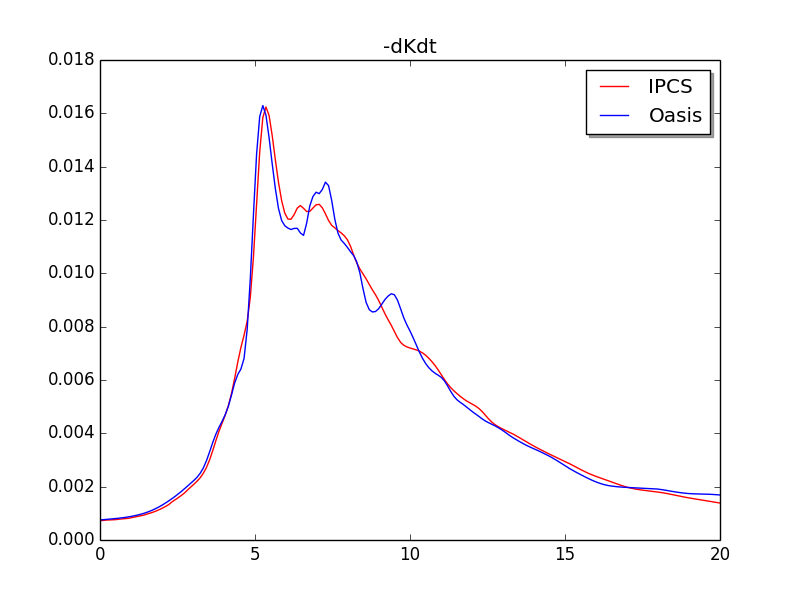
\includegraphics[scale=0.4]{./Verification_Validation/TaylorGreen/Dkdt.png}
  \captionof{figure}{$\epsilon(E_k)$ N = 32}
  \label{fig:test1}
\end{minipage}%
\begin{minipage}{.5\textwidth}
  \centering
  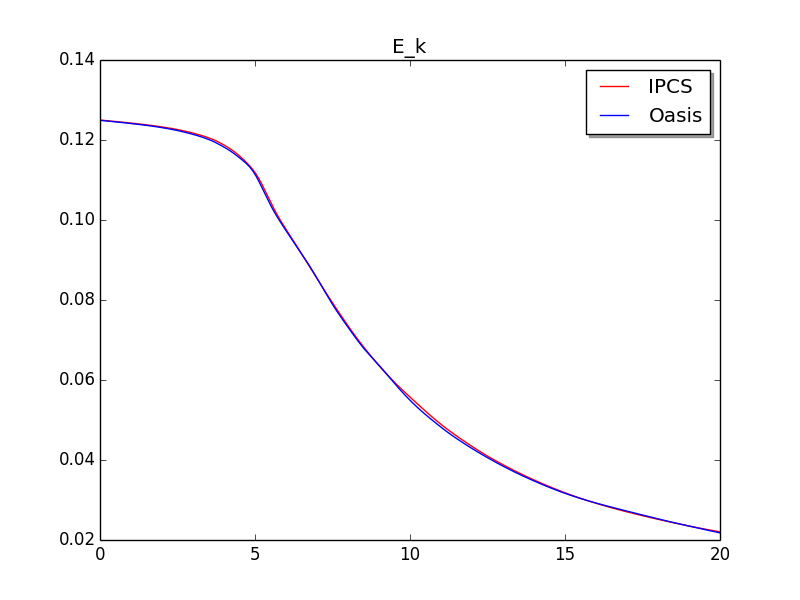
\includegraphics[scale=0.4]{./Verification_Validation/TaylorGreen/Ek.png}
  \captionof{figure}{$E_k$ N = 32 }
  \label{fig:test2}
\end{minipage}
\end{figure}
\end{center}



































\section*{Fluid-Structure Interaction between an elastic object and laminar incompressible flow}
The goal of this benchmark is to test the fluid and solid solver first separately and then together as a full FSI problem \cite{Hron2006a}. This benchmark is based on the older benchmark \" flow around cylinder\" with fluid considered incompressible and in the laminar regime, and the structure deformations are significant. The problem is setup with the solid submerged in the fluid, so that oscillations in the fluid deform the structure. We will measure the drag and lift around the circle and bar, and measure structural displacement at a given point. 

\subsection*{Problem Defintion}
\subsubsection*{Domain}
\begin{center}
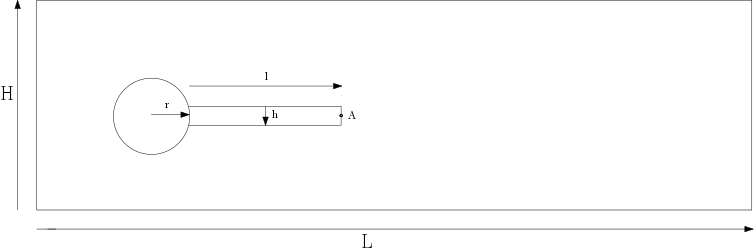
\includegraphics[scale=0.4]{./Verification_Validation/Hron_Turek/Domain_drawing.png}
\end{center}
The computational domain consists of a circle with an elastic bar behind the circle. The circle is positioned at (0.2, 0.2) making it 0.05 of center from bottom to top, this is done to induce oscillations to an otherwise laminar flow. 
This gives a force to the elastic bar. The parameters of the domain are:\\
L = 2.5, H = 0.41, l = 0.35, h = 0.02, A = (0.2,0.6) \\

\subsubsection*{Boundary conditions}
The fluid velocity has a parabolic profile on the inlet that changes over time:\\

\begin{align*}
u(0,y) &= 1.5u_0 \frac{y(H-y)}{(\frac{H}{2})^2}  \\
u(0,y,t) &= u(0,y)\frac{1-cos(\frac{\pi}{2}t)}{2} \text{  for  } t<2.0 \\
u(0,y,t) &= u(0,y) \text{  for  } t \leq 2.0
\end{align*}

We set no slip on the "floor" and "ceiling" so to speak.\\
$$ u(x,y,t) = 0 \text{  on  }  $$
On the fluid solid interface the boundary conditions are set to:
$$  \sigma_f n_f = \sigma_s n_s \hspace{4mm} on  \hspace{2mm}\Gamma^0 (interface)   $$
In our variational form we leave this out and so implying that they are equal.

\subsubsection*{Quantities for comparison}
When the fluid moves around the circle and bar it exerts a force. These are split into drag and lift and calculated as follows:
$$ (F_d, F_L) = \int_S \sigma_f n dS $$ 
where S is the part of the circle and bar in contact with the fluid. \\
We set a point A on the right side of the bar. This point is used to track the deformation in CSM and FSI tests. \\
In each test the numbers with ref are the values taken from the benchmark paper \cite{Hron2006a}
We integrate the mapped fluid stress tensor over the bar and circle and appended to lists: 
\begin{lstlisting}[language=Python]
Dr = -assemble((sigma_f_new(v,p,d,mu_f)*n)[0]*ds(6))
Li = -assemble((sigma_f_new(v,p,d,mu_f)*n)[1]*ds(6))
Dr += -assemble((sigma_f_new(v("-"),p("-"),d("-"),mu_f)*n("-"))[0]*dS(5))
Li += -assemble((sigma_f_new(v("-"),p("-"),d("-"),mu_f)*n("-"))[1]*dS(5))
Drag_list.append(Dr)
Lift_list.append(Li)
\end{lstlisting}
The deformation is calculated on the point A, and also added to lists:
\begin{lstlisting}[language=Python]
dsx = d(coord)[0]
dsy = d(coord)[1]
dis_x.append(dsx)
dis_y.append(dsy)
\end{lstlisting}
\subsection{Results}
\subsubsection*{CFD test}
The first two CFD tests are run with Reynolds number 20 and 100 giving steady drag and lift around the circle. CFD 3 has a Reynolds number 200 which will induce oscillations behind the circle, giving fluctuations in the drag and lift.
The CFD tests were run using the the bar as rigid object, that is the domain calculated is just the fluid domain. It is possible to also calculate with the bar and setting $\rho_s$ and $\mu_s$ to a large value. 

\begin{table}[h!]
\centering
\caption{CFD parameters}
\label{my-label}
\begin{tabular}{|l|l|l|l|}
\hline
Parameters & CFD1 & CFD2 & CFD3 \\ \hline
$\rho_f [10^3 \frac{kg}{m^3}]$ & 1 & 1 & 1 \\ \hline
$\nu_f [10^{-3} \frac{m^2}{s}]$ & 1 & 1 & 1 \\ \hline
$ U [\frac{m}{s}] $ & 0.2 & 1 & 2 \\ \hline
Re = $\frac{Ud}{\nu_f}$ & 20 & 100 & 200 \\ \hline
\end{tabular}
\end{table}

\begin{table}[h!]
\centering
\caption{CFD 1}
\label{my-label}
\begin{tabular}{|l|l|l|l|}
\hline
\textbf{elements} & \textbf{dofs} & \textbf{Drag} & \textbf{Lift} \\ \hline
6616 & 32472 & 14.2439 & 1.0869 \\ \hline
26464 & 124488 & 14.2646 & 1.11085 \\ \hline
105856 & 487152 & 14.2755 & 1.11795 \\ \hline
\textbf{ref} & \textbf{} & \textbf{14.29} & \textbf{1.119} \\ \hline
\end{tabular}
\end{table}

\begin{table}[h!]
\centering
\caption{CFD 2}
\label{my-label}
\begin{tabular}{|l|l|l|l|}
\hline
\textbf{elements} & \textbf{dofs} & \textbf{Drag} & \textbf{Lift} \\ \hline
6616 & 32472 & 135.465 & 6.27158 \\ \hline
26464 & 124488 & 136.566 & 9.82166 \\ \hline
105856 & 487152 & 136.573 & 10.4441 \\ \hline
\textbf{ref} & \textbf{} & \textbf{136.7} & \textbf{10.53} \\ \hline
\end{tabular}
\end{table}

\subsubsection*{CSM test}
The CSM test are calculated using only the bare and adding a gravity term $g$ with the same value but changing the parameters of solid.
As with the CFD test the first to CSM test cause a steady state solution, and CSM 3 is more slender causing the bar to go up and down in time. Our quantity for comparing there will be the deformation of the point $A$. In CSM 3 the energy is conserved by using a Crank-Nicholson scheme as can be seen in the plots fig7 (hvordan citer man et plot?)

\begin{table}[h!]
\centering
\caption{Parameters}
\label{my-label}
\begin{tabular}{|l|l|l|l|}
\hline
Parameters & CSM1 & CSM2 & CSM3 \\ \hline
$\rho_f[10^3 \frac{kg}{m^3}]$ & 1 & 1 & 1 \\ \hline
$\nu_f [10^{-3} \frac{m^2}{s}]$ & 1 & 1 & 1 \\ \hline
$u_0$ & 0 & 0 & 0 \\ \hline
$\rho_s[10^3 \frac{kg}{m^3}]$ & 1 & 1 & 1 \\ \hline
$\nu_s$ & 0.4 & 0.4 & 0.4 \\ \hline
$\mu_s[10^6 \frac{m^2}{s}]$ & 0.5 & 2.0 & 0.5 \\ \hline
$g $ & 2 & 2 & 2 \\ \hline
\end{tabular}
\end{table}

\begin{table}[h!]
\centering
\caption{CSM 1}
\label{my-label}
\begin{tabular}{|l|l|l|l|}
\hline
elements & dofs & ux $[10^{?3}]$ & uy $[10^{?3}]$ \\ \hline
725 & 1756 & -5.80951654915 & -59.4781430115 \\ \hline
2900 & 6408 & -6.77960453995 & -64.2130757639 \\ \hline
11600 & 24412 & -7.08597041285 & -65.635825349 \\ \hline
46400 & 95220 & -7.11626976966 & -65.7456687273 \\ \hline
ref & ref & -7.187 & -66.10 \\ \hline
\end{tabular}
\end{table}

% Please add the following required packages to your document preamble:
% \usepackage{booktabs}
\begin{table}[h!]
\centering
\caption{CSM 2}
\label{my-label}
\begin{tabular}{@{}|l|l|l|l|@{}}
\hline
Elements & Dofs & ux $[10^{-3}] $& ux $[10^{-3}] $\\ \hline
725 &  1756 & -0.375962146908 & -15.1950342598 \\ \hline
2900 & 6408 & -0.441308781709 & -16.4643196042\\ \hline
11600 & 24412 & -0.462087305294 & -16.8478689583 \\ \hline
46400 & 95220 & -0.464128022327 & -16.8782135872\\ \hline
ref & ref & -0.4690 & -16.97 \\ \hline
\end{tabular}
\end{table}

\begin{table}[h!]
\centering
\caption{CSM 3}
\label{my-label}
\begin{tabular}{|l|l|l|l|}
\hline
elements & dofs & ux $[10^3]$ & uy $[10^3]$ \\ \hline
725 & 1756 & $-11.743 \pm 11.744$ & $-57.952 \pm 58.940$ \\ \hline
2900 & 6408 & $-13.558 \pm 13.559$ & $ -61.968 \pm  63.440 $ \\ \hline
11600 & 24412 & $ -14.128 \pm 14.127$ & $-63.216 \pm 64.744 $ \\ \hline
46400 & 95220 & $ -14.182 \pm 14.181 $ & $ -63.305 \pm 64.843 $ \\ \hline
ref &  & $-14.305 \pm 14.305 $ & $-63.607 \pm 65.160 $ \\ \hline
\end{tabular}
\end{table}

\begin{figure}[h!] 
  \begin{subfigure}[b]{0.5\linewidth}
    \centering
    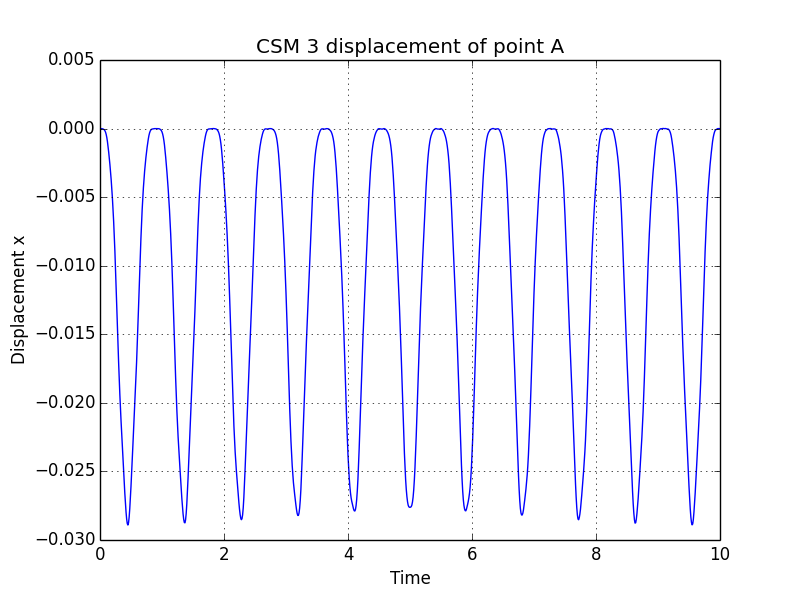
\includegraphics[width=0.75\linewidth]{./Verification_Validation//Hron_Turek/dis_x.png} 
    \caption{Displacement in x-direction} 
    \label{fig7:a} 
    \vspace{4ex}
  \end{subfigure}%% 
  \begin{subfigure}[b]{0.5\linewidth}
    \centering
    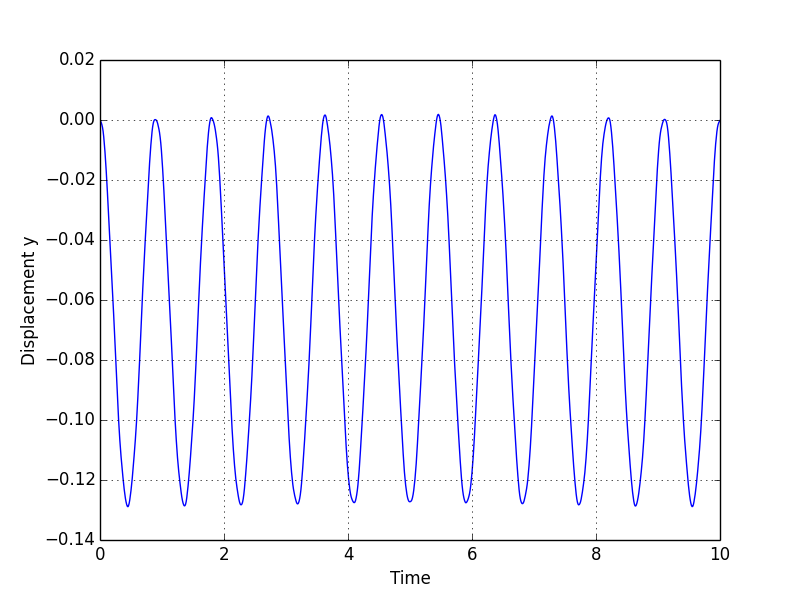
\includegraphics[width=0.75\linewidth]{./Verification_Validation//Hron_Turek/dis_y.png} 
    \caption{Displacement in x-direction} 
    \label{fig7:b} 
    \vspace{4ex}
  \end{subfigure} 
  \begin{subfigure}[b]{0.5\linewidth}
    \centering
    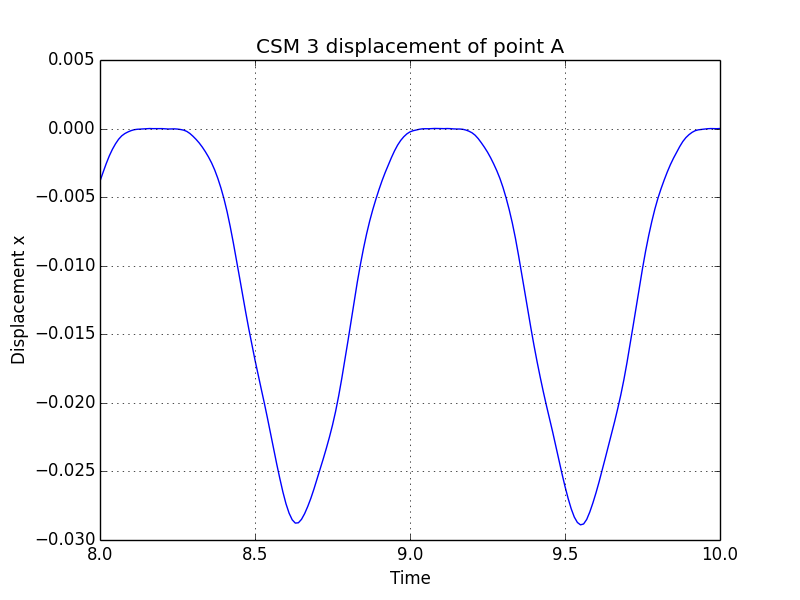
\includegraphics[width=0.75\linewidth]{./Verification_Validation//Hron_Turek/dis_x_short.png} 
    \caption{Displacement in x-direction} 
    \label{fig7:c} 
  \end{subfigure}%%
  \begin{subfigure}[b]{0.5\linewidth}
    \centering
    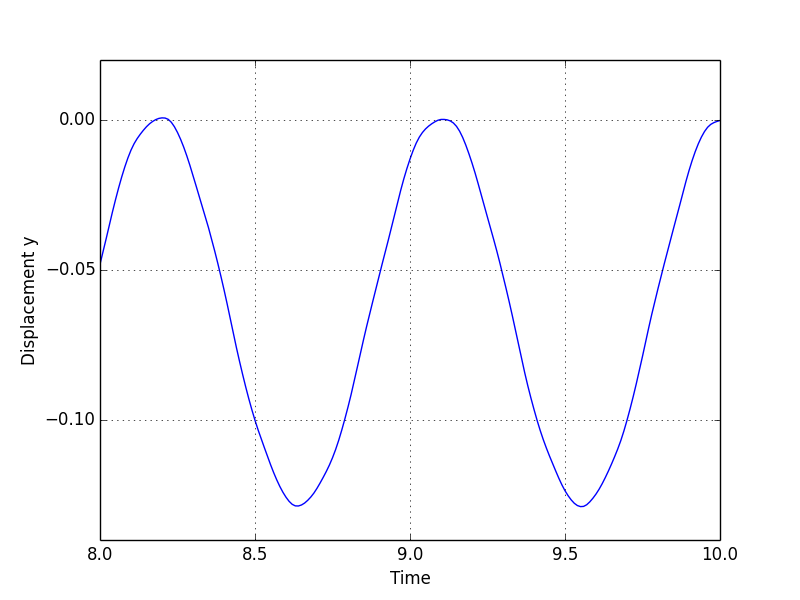
\includegraphics[width=0.75\linewidth]{./Verification_Validation/Hron_Turek/dis_y_short.png} 
    \caption{Displacement in x-direction} 
    \label{fig7:d} 
  \end{subfigure} 
  \caption{Displacement of point A}
  \label{fig7} 
\end{figure}


\subsection*{FSI test}
\begin{table}[ht]
\centering
\caption{FSI Parameters}
\label{my-label}
\begin{tabular}{|l|l|l|l|}
\hline
Parameters & FSI1 & FSI2 & FSI3 \\ \hline
$\rho_f[10^3 \frac{kg}{m^3}]$ & 1 & 1 & 1 \\ \hline
$\nu_f [10^{-3} \frac{m^2}{s}]$ & 1 & 1 & 1 \\ \hline
$u_0$ & 0.2 & 1 & 2 \\ \hline
Re = $\frac{U d}{\nu_f}$ & 20 & 100 & 200 \\ \hline
$\rho_s[10^3 \frac{kg}{m^3}]$ & 1 & 10 & 1 \\ \hline
$\nu_s$ & 0.4 & 0.4 & 0.4 \\ \hline
$\mu_s[10^6 \frac{m^2}{s}]$ & 0.5 & 0.5 & 2 \\ \hline
\end{tabular}
\end{table}
Results: 
\begin{table}[h]
\centering
\caption{FSI 1}
\label{my-label}
\begin{tabular}{|l|l|l|l|l|l|l|}
\hline
Cells & Dofs & ux of A $[x10^{-3}]$ & uy of A $[x10^{-3}]$ & Drag & Lift & Spaces \\ \hline
2698 & 7095 & 0.0234594 & 0.797218  & 14.4963 & 0.915801 & P1-P1-P1 stab= 0.01 \\ \hline
2698 & 23563 &0.0227418 &0.799314  &  14.1735 &0.761849 & P2-P2-P1 \\ \hline
10792 & 92992  &0.0227592 & 0.80795 & 14.1853 &  0.775063 &  P2-P2-P1 \\ \hline
43168 & 369448 & 00.227566 & 0.813184 & 14.2269 & 0.771071 & P2-P2-P1 \\ \hline
\textbf{ref} & \textbf{ref} & \textbf{0.0227} & \textbf{0.8209} & \textbf{14.295} & \textbf{0.7638} & \textbf{ref} \\ \hline
\end{tabular}
\end{table}



\newpage
OLD SHITZ FSI:
\begin{table}[h]
\centering
\caption{FSI 1}
\label{my-label}
\begin{tabular}{|l|l|l|l|l|l|l|}
\hline
Cells & Dofs & ux of A $[x10^{-3}]$ & uy of A $[x10^{-3}]$ & Drag & Lift & Spaces \\ \hline
2698 & 7095 & 0.0234594 & 0.797218  & 14.4963 & 0.915801 & P1-P1-P1 stab= 0.01 \\ \hline
2698 & 23563 & 0.02271 & 0.80288 & 14.1736 & 0.787891 & P2-P2-P1 \\ \hline
2698 & 23563 & 0.00581116 & 0.000000738678  & 12.07 & 0.02345 & P2-P2-P1 without weighting \\ \hline
10792 & 92992 & 0.0227341 & 0.808792 & 14.1855 & 0.801044 & P2-P2-P1 \\ \hline
43168 & 369448 & 0.227352 & 0.812595 & 14.227 & 0.797242 & P2-P2-P1 \\ \hline
\textbf{ref} & \textbf{ref} & \textbf{0.0227} & \textbf{0.8209} & \textbf{14.295} & \textbf{0.7638} & \textbf{ref} \\ \hline
\end{tabular}
\end{table}









